\chapter{Commande temps discret}
Afin d'implémenter la commande,  nous allons adapter la commande de façon à ce qu'elle soit implémentable sur le micro-contrôleur. Ensuite, nous évaluerons cette transformation. Voici, ci-dessous figure \ref{fig:GeneralSCHEMA}, le schéma général des différents éléments.	

	  	
	  	
	  	

\section{Discrétisation de la commande}
Nous allons à présent transformer la commande en temps continue en une forme qui permet l'implémentation sur un micro-contrôleur. Nous avons choisi de l'implémenter sous la forme d'une équation récurrente. Pour cela, dans un premier temps, nous avons transformer la commande (composée d'un observateur, d'un retour d'état et d'un pré-compensateur) en une forme espace d'états puis nous la discrétiserons. Ensuite, nous allons la transformer en une fonction de transfert pour finalement la transformer en équation récurrente.
	\subsection{Espace d'état à temps discret de la commande}
%		 (observateur + retour état = 2 ft)
%1. obs + re = EE
La commande est de la forme suivante (figure \ref{fig:comTC}) : 
\begin{figure}[!ht]
\centering
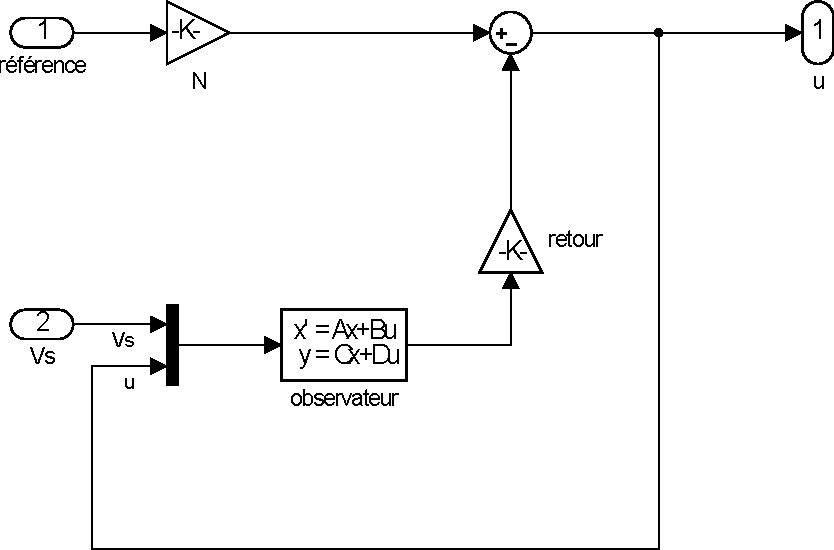
\includegraphics[width=.4\textwidth]{./V/images/Com_asserv.pdf}
\caption{\label{fig:comTC}Schéma de la commande par retour d'état à temps continue.}
\end{figure}


Voici, issue des équations \ref{equ:obs} et \ref{equ:obs2}, l'observateur simplifié (équation \ref{equ:obsSimp}).
\begin{equation}
\label{equ:obsSimp}
\left\lbrace
\begin{aligned}
&\dot z (t) = Fz(t) + GV_S(t) + Bu(t)\\
&\hat{x}(t) = z(t)
\end{aligned}
\right.
\end{equation}
Ainsi que le retour d'état :
\begin{equation}
u(t) = -K\hat{x}(t) + N V_{ref}(t)
\end{equation}
Nous allons rassembler ces équations afin de créer un nouvel espace d'état:
\begin{equation}
\begin{array}{ll}
&\left\lbrace
\begin{aligned}
&\dot z (t) = Fz(t) + GV_S(t) + Bu(t)\\
&u(t) = -Kz(t) + N V_{ref}(t)
\end{aligned}
\right.
\Leftrightarrow
\left\lbrace
\begin{aligned}
&\dot z (t) = (F-KB)z(t) + GV_S(t) + BN V_{ref}(t)\\
&u(t) = -Kz(t) + N V_{ref}(t)
\end{aligned}
\right.\\
&\\

\Leftrightarrow&
\left\lbrace
\begin{aligned}
&\dot z (t) = (F-KB)z(t) + 
\begin{bmatrix} G &  BN \end{bmatrix}  
\begin{bmatrix} V_S(t) \\ V_{ref}(t)  \end{bmatrix}  
\\
&u(t) = -Kz(t) + 
\begin{bmatrix} N &  0 \end{bmatrix}  
\begin{bmatrix} V_S(t) \\ V_{ref}(t)  \end{bmatrix}  
\end{aligned}
\right.
\end{array}
\end{equation}
%2. EE(z)
Maintenant que nous avons exprimer la commande sous la forme d'un espace d'état, avec pour entrées $V_{ref}(t)$ la consigne et $V_S(t)$, la sortie de position mesurée, nous pouvons discrétisé la commande. Nous avons choisis de discrétiser la commande grâce à matlab, avec l'option \emph{tustin} afin d'avoir une commande la plus fidèle possible à celle en temps continue.
Cela donne la commande à temps discret suivante :
\begin{equation}
\label{equ:EEcomTD}
\begin{array}{rl}
& \left\lbrace
\begin{array}{rclcl}
z(z-1) 	&=& A z(z) &+& B \begin{bmatrix} V_S(t) \\ V_{ref}(t)  \end{bmatrix}  \\
u(z)  	&=& C z(z) &+& D \begin{bmatrix} V_S(t) \\ V_{ref}(t)  \end{bmatrix}  
\end{array}
\right.\\
&\\
\Leftrightarrow &
\left\lbrace
\begin{array}{rclcclc}
z(z-1) 	&=& 
\begin{bmatrix}
0.7679 		&  0.03725\\
-0.00193   	& 0.6207
\end{bmatrix} &z(z) 
&+& \begin{bmatrix}
0.08301  &  0.2089\\
3.612  	 &	0.001737
\end{bmatrix} 
&\begin{bmatrix} V_S(t) \\ V_{ref}(t)  \end{bmatrix}  \\
u(z)  	&=& \begin{bmatrix}
8.589*10^{-05}  &  -0.07211
\end{bmatrix} &z(z) &+& \begin{bmatrix}
1.35  & -7.73*10^{-05}
\end{bmatrix} 
&\begin{bmatrix} V_S(t) \\ V_{ref}(t)  \end{bmatrix}  
\end{array}
\right.
\end{array}
\end{equation}
	\subsection{Équation récurrente}
%1. EE 		= 2*tf(z)
	Nous allons maintenant transformer l'espace d'état de l'équation \ref{equ:EEcomTD} en fonctions de transferts, à l'aide de matlab :
\begin{eqnarray}
\frac{u(z)}{V_s(z)} &=& \frac{1.35 z^2 - 2.135 z + 0.8435}{    z^2 - 1.389 z + 0.4767}\\
\frac{u(z)}{V_{ref}(z)}	&=&	\frac{-7.73*10^{-05} z^2 - 8.582*10^{-21} z + 7.73*10^{-05}}{z^2 - 1.389 z + 0.4767}
\end{eqnarray}

%2. 2*tf(z) = 1*tf(z^-1)

Afin d'avoir une commande causale, nous avons passer les fonctions de transferts en $z^{-1}$ :
\begin{eqnarray}
\label{equ:ftTD1}\frac{u(z^{-1})}{V_s(z^{-1})} &=& \frac{1.35  - 2.135 z^{-1} + 0.8435 z^{-2}}{    1 - 1.389 z^{-1} + 0.4767 z^{-2}}\\
\label{equ:ftTD2}\frac{u(z^{-1})}{V_{ref}(z^{-1})}	&=&	\frac{-7.73*10^{-05} - 8.582*10^{-21} z^{-1} + 7.73*10^{-05} z^{-2}}{    1 - 1.389 z^{-1} + 0.4767 z^{-2}}
\end{eqnarray}
Nous avons ensuite, à partir des équations \ref{equ:ftTD1} et  \ref{equ:ftTD2}, créer une seule équation :
\begin{equation}
\label{equ:eqTDz-}
\begin{array}{lcl}
u(z^{-1})(1 - 1.389 z^{-1} + 0.4767 z^{-2}) &=& (1.35  - 2.135 z^{-1} + 0.8435 z^{-2})  V_s(z^{-1}) \\
&&+ (-7.73*10^{-05} - 8.582*10^{-21} z^{-1} + 7.73*10^{-05} z^{-2})V_{ref}(z^{-1})
\end{array}
\end{equation}
Nous avons maintenant une seule équation pour représenter la commande à temps discret.%
%3. tf(z^-1)= ER(z^-1)
Il faut maintenant la transformée en équation récurrente, pour cela nous allons utiliser la propriété suivante :
\begin{equation}
f(z)z^n = f_{k+n}
\end{equation}
Cela donne, une fois réorganiser de façon a isoler la sortie $u_k$ et à partir de l'équation \ref{equ:eqTDz-} :
\begin{equation}
\begin{array}{lcl}
u_k &=&  1.389 u_{k-1} - 0.4767 u_{k-2} + 1.35Vs_{k}  - 2.135 Vs_{k-1} + 0.8435 Vs_{k-2}  \\
&& -7.73*10^{-05}Vr_k - 8.582*10^{-21} Vr_{k-1} + 7.73*10^{-05} Vr_{k-2}
\end{array}
\end{equation}
Où,par soucis de lisibilité, $Vs = V_s$ et $Vr = V_{ref}$.
Le coût temporel de ce calcul est au minimum de $8*400ns = 3,2 ms$.
Maintenant que nous avons une équation implémentable sur micro contrôleur, il faut créer un code le permettant, à partir de celui fourni.
